\documentclass{article} 
\usepackage{tikz}
\usetikzlibrary{patterns}
\usetikzlibrary{decorations.shapes}
\usetikzlibrary{intersections}
\usetikzlibrary{shapes,arrows,shadows,positioning}
\usetikzlibrary{backgrounds}


\usepackage{pagecolor}


\definecolor{mathlab-orange}{HTML}{FE9800}%
\definecolor{mathlab-blue}{HTML}{07549A}%


\begin{document}

\pagecolor{mathlab-blue}

\begin{figure}
\centering
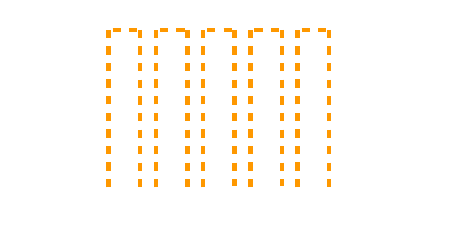
\begin{tikzpicture}
\draw[-, ultra thick, color=white] (4.8,0) -- (4.8,2);
\draw[-, ultra thick, color=white] (4.8,2) -- (8,2);
\draw[-, ultra thick, color=white] (8,2) -- (8,0);
\draw[->, ultra thick, color=white] (4,0) -- (8.8,0) node[right] {$t$};
\draw[dashed, color=mathlab-orange, ultra thick] (5,0.03) -- (5,2.03);
\draw[dashed, color=mathlab-orange, ultra thick] (5.05,2.03) -- (5.4,2.03);
\draw[dashed, color=mathlab-orange, ultra thick] (5.4,2.03) -- (5.4,0.03);
\draw[dashed, color=mathlab-orange, ultra thick] (5.6,0.03) -- (5.6,2.03);
\draw[dashed, color=mathlab-orange, ultra thick] (5.65,2.03) -- (6,2.03);
\draw[dashed, color=mathlab-orange, ultra thick] (6,2.03) -- (6,0.03);
\draw[dashed, color=mathlab-orange, ultra thick] (6.2,0.03) -- (6.2,2.03);
\draw[dashed, color=mathlab-orange, ultra thick] (6.25,2.03) -- (6.6,2.03);
\draw[dashed, color=mathlab-orange, ultra thick] (6.6,2.03) -- (6.6,0.05);
\draw[dashed, color=mathlab-orange, ultra thick] (6.8,0.03) -- (6.8,2.03);
\draw[dashed, color=mathlab-orange, ultra thick] (6.85,2.03) -- (7.2,2.03);
\draw[dashed, color=mathlab-orange, ultra thick] (7.2,2.03) -- (7.2,0.05);
\draw[dashed, color=mathlab-orange, ultra thick] (7.4,0.03) -- (7.4,2.03);
\draw[dashed, color=mathlab-orange, ultra thick] (7.45,2.03) -- (7.8,2.03);
\draw[dashed, color=mathlab-orange, ultra thick] (7.8,2.03) -- (7.8,0.03);
%\draw [decorate,decoration={brace,raise=2pt}, color=red] (4.8,2.6) -- (8,2.6) node [midway,above=1pt] {$\phi(\boldsymbol{\mu}), C_p(\boldsymbol{\mu})$};
%\draw [decorate,decoration={brace,raise=1pt}] (5,2.03) -- (5.4,2.03) node [midway,above=1pt] {$\phi_N(\boldsymbol{\mu}), C_p^N(\boldsymbol{\mu})$};
\end{tikzpicture}
\end{figure}

\begin{figure}
\centering
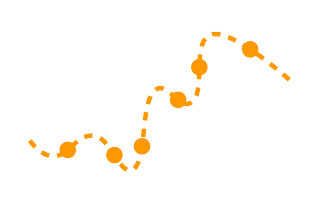
\begin{tikzpicture}
\draw [white, name path=line 1, ultra thick] plot [smooth, tension=1] coordinates { (-0.32,-0.38) (1,-0.62) (2,0.55) (3,0.45)};
\draw [mathlab-orange, name path=line 2, ultra thick, dashed] plot [smooth, tension=0.8] coordinates { (-0.32,-0.5) (0,-0.7) (0.5, -0.44) (1,-0.86) (1.25, 0.12) (1.75, -0) (2,0.85) (3,0.25)};
%\begin{scope}[on background layer]
\fill[mathlab-orange,name intersections={of=line 1 and line 2,total=\t}]
    \foreach \s in {1,...,\t}{(intersection-\s) circle (3pt)};
%\end{scope}
\end{tikzpicture}
\end{figure}

\end{document}



